\documentclass[12pt,a4paper]{article}
\usepackage{rotating}
\usepackage[utf8]{inputenc}
\usepackage{amsmath, amssymb}
\usepackage{graphicx}
\usepackage{hyperref}
\usepackage{fancyvrb}

\usepackage{listings}
\usepackage{xcolor}

\title{Formula 1 Data Analysis Project \\
    \large Machine learning to predict the best strategy for a F1 race
}
\author{Martino Papa}
\date{\today}

\lstset{
    basicstyle=\ttfamily\footnotesize,
    breaklines=true,
    frame=single,
    backgroundcolor=\color{gray!10},
    keywordstyle=\color{blue},
    commentstyle=\color{green!50!black},
    stringstyle=\color{red!60!black}
}

\begin{document}

\maketitle

\section{Introduction}
The goal of this project is to predict the best strategy for a Formula 1 race. To do so we will use the data provided by the free-practice sessions to train a machine learning model that will predict the laptimes. Then we will use those predictions to simulate a race and find the best strategy.  

This project aims to analyze Formula~1 telemetry and lap time data using the \texttt{FastF1} Python library.
The core of the project is developed in the notebook \texttt{f1.ipynb}, which leverages two custom Python modules: 
\texttt{f1Analysis.py} for data retrieval, preprocessing, and clustering, and \texttt{mesures.py} for evaluation metrics.

\section{Dataset Description}
The dataset is accessed via the \texttt{FastF1} library, which provides an interface to Formula~1 telemetry data. The primary function used to retrieve the data is:
\\\textbf{Function:} \verb|get_data(year, event, session_name)|
\textbf{Description:}  
Retrieves telemetry and session information from the \texttt{FastF1} database for a given Formula~1 race weekend session. The method loads data such as lap times, stint information, weather data, and track status.
\textbf{Parameters:}
\begin{itemize}
    \item \verb|year| \quad (integer) \\
    The year of the Formula~1 season.  
    Example: \verb|2024|.
    
    \item \verb|event| \quad (string or integer) \\
    The race event identifier. This can be either the name of the Grand Prix (e.g.\ \verb|"Japan"|) or the round number (e.g.\ \verb|4| for the fourth race of the season).
    
    \item \verb|session_name| \quad (string) \\
    The name of the session to load. Common options include:
    \verb|"FP1"|, \verb|"FP2"|, \verb|"FP3"|, \verb|"Q"| (Qualifying), \verb|"SQ"| (Sprint Qualifying), \verb|"S"| (Sprint), \verb|"R"| (Race).
\end{itemize}
\noindent
\textbf{Returns:}  
A \verb|Session| object containing structured data for the selected session with the following attributes.
\textit{
Time,
Driver,
DriverNumber,
LapTime,
LapNumber,
Stint,
PitOutTime,
PitInTime,
Sector1Time,
Sector2Time,
Sector3Time,
Sector1SessionTime,
Sector2SessionTime,
Sector3SessionTime,
SpeedI1,
SpeedI2,
SpeedFL,
SpeedST,
IsPersonalBest,
Compound,
TyreLife,
FreshTyre,
Team,
LapStartTime,
LapStartDate,
TrackStatus,
Position,
Deleted,
DeletedReason,
FastF1Generated,
IsAccurate.
}

\noindent
To make our predictions we will use all the 3 free practice sessions (FP1, FP2 and FP3) and we will extrapolate the following extra features (this is done by the method \verb|get_data()| contained in \texttt{f1Analysis.py}):
\textit{LapsInStint
OutLap
InLap
FuelLevel
Session}.

In this project we will focus on the 2024 Japanese Grand Prix, in this case the dataset will contain 647 laps considering all the 3 free practice sessions. The first goal is to identify the ``clean'' laps, i.e.\ the laps that are representative of the car's performance and not of drivers mistakes or unusual track conditions.

\section{Cleaning the dataset}
First we remove the laps that are marked as InLaps or OutLaps, then we perform a Clustering analysis to identify the clean laps.
\subsection{Clustering}
To distinguish clean laps from unrepresentative ones, clustering methods are applied:
\begin{itemize}
    \item \textbf{DBSCAN} — density-based clustering robust to noise.
    \item \textbf{KMeans} — partition-based clustering.
\end{itemize}
Both algorithms are implemented in the \texttt{f1Analysis.py} module. The clustering is performed on the sector times of each lap in regard to reward consistency across sectors. Because of the need to identfy driver mistakes we will use chebyshev distance as metric for both algorithms, this will penalize more the mistakes since there will be a big only in one sector and not in the other 2.
Parameters are tuned by evaluating the quality of the largest cluster with the metric defined in \texttt{mesures.py}. It's important to notice that this works under the assumpion that most of the laps will be clean ones. 

The two clustering techniques return very similar results in the case of the Japanese Grand Prix. We choose to keep only the laps that are classified as clean by both algorithms, this will ensure a higher quality of the selected laps. After this phase we are left with 235 laps in our dataset.
\begin{figure}
    \centering
    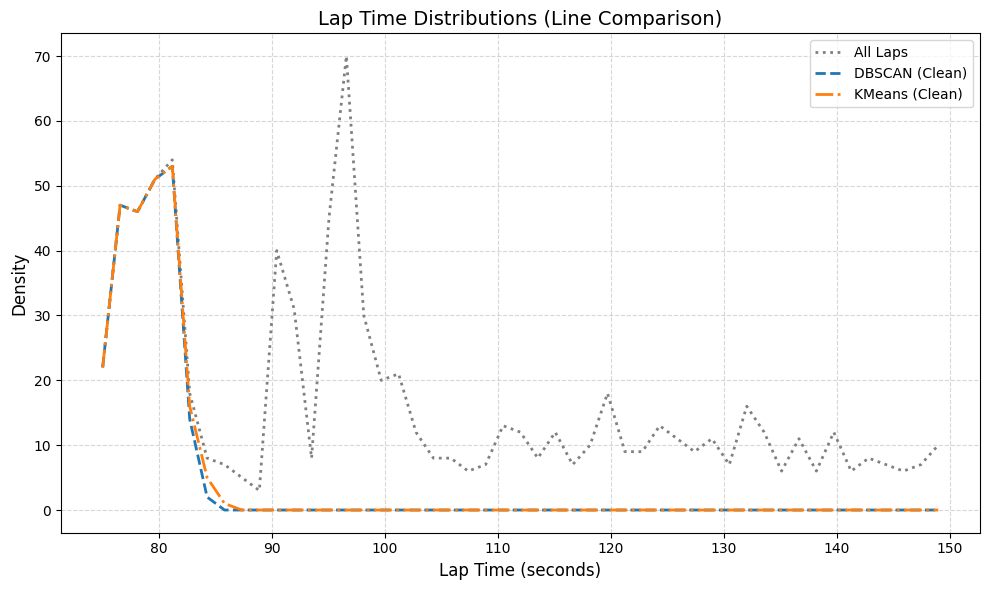
\includegraphics[width=1\textwidth]{lap_distribution.png}
    \caption{Clustering results}
    \label{fig:clustered_laps}
\end{figure}
We them perform a final cleaning step by removing the laps with a high variance in sector times, this is done to remove the laps that are not consistent across sectors. This leaves us with 230 laps to work with. This number is sufficient to train a simple machine learning method (eg. decision trees), but defintly not enough to build an efficient neural network. Fourther implementations should considering using the data from previous years to improve the predictions.

\section{Predicting the lap times}
After the preprocessing phase we can now jump to the prediction of the lap times. To do so we will use the following features:
\begin{itemize}
    \item \textbf{Compound} \(\in \{"HARD", "MEDIUM", "SOFT"\}\)\ which will be encoded with an ordinal encoder since the compounds have a natural order.
    \item \textbf{TyreLife}, which is the number of laps done with the current set of tyres.
    \item \textbf{FuelLevel}, which is the amount of fuel in the car at the start of the lap. The dataset doesn't provide this feature but it can be estimated knowing the number of laps in the stint.
    \item \textbf{Session} \(\in \{"FP1", "FP2", "FP3"\}\)\ which will be encoded with an ordinal encoder since the track should improve trough the sessions.
\end{itemize}
To predict the lap times we tested 3 different models: decision tree, neural networks and random forest. The results are summarized in the table below:
\begin{table}[h!]
    \centering
    \begin{tabular}{|c|c|c|}
        \hline
        Model & MSE training & MSE test \\
        \hline
        Decision Tree & 1.82 & 2.39 \\
        Neural Network & 2.20 & 2.95 \\
        Random Forest & 1.15 & 1.98 \\
        \hline
    \end{tabular}
    \caption{Model performance comparison}
    \label{tab:model_performance}
\end{table}

NB: the tuning results are not shown here for brevity, they can be found in the notebook \texttt{f1.ipynb}.

The random forest seems to be the best model here and we will use it to predict the laptimes during the race simulation that we will perform to compute the best strategy. Altough the decision tree seems to be less precise it's intresting to analyze how it makes the predictions, this can be done by visualizing the tree structure Figure \ref{fig:decision_tree}).
\begin{sidewaysfigure}
    \centering
    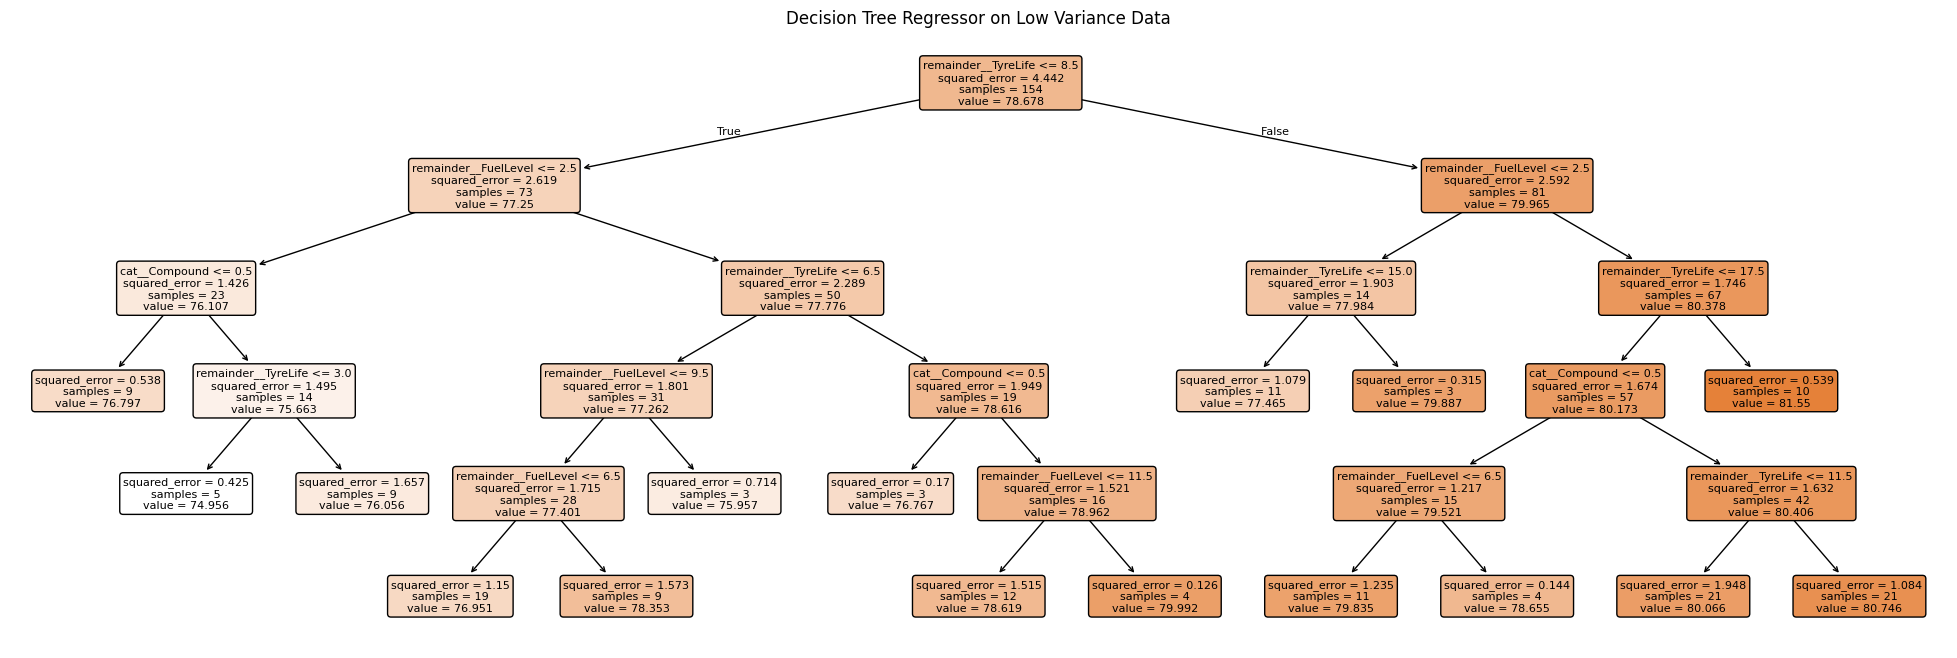
\includegraphics[width=1\textheight,keepaspectratio]{decision_tree.png}
    \caption{Decision tree structure}
    \label{fig:decision_tree}
\end{sidewaysfigure}

We also add the feature importance plot (Figure \ref{fig:feature_importance}) made by the random forest to understand which features are more important for the predictions. It's intresting to notice that the session has zero importance on the prediction, so the assumpion of the track improvment trough the sessions is not valid in this case.

A MSE of 1.98 comes with an average error in the lap time prediction of 1.15 seconds, which is acceptable for our purpose. We have to keep in mind that due to the lack of data we are predicting the same time for all the cars and drivers, when in the reality there are big differences between drivers and teams.
\begin{figure}
    \centering
    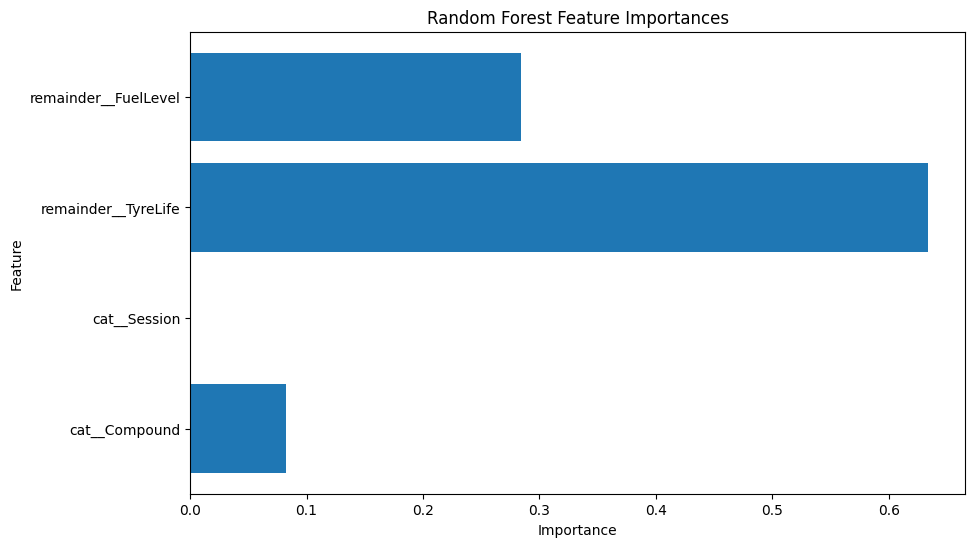
\includegraphics[width=1\textwidth]{featureimp.png}
    \caption{Random forest feature importance}
    \label{fig:feature_importance}
\end{figure}

\section{Computing the best strategy}
To compute the best strategy we will use a \texttt{backtracking} algorithm that will explore all the possible strategies using the random forest model to predict lap times. It's important to apply \texttt{Memoization} to avoid recomputing the same strategy multiple times. The algorithm is implemented in the method \verb|best_strategy()| contained in \texttt{f1Analysis.ipynb}.
The algorithm explores all the possible strategies with a maximum of 5 stops, this is done to limit the number of strategies to explore and takes into account the pit stop time, which is set to 23.545 seconds for the Japanese Grand Prix and the number of laps in the race (53). It also needs to satisfy the tyre rule constraint, which states that each driver must use at least 2 different compounds during the race. The results are the following:

\begin{Verbatim}[frame=single, fontsize=\footnotesize , xleftmargin=1em]
Best total time: 4213.0599 seconds

Best strategy:
Lap   Action   Compound   Predicted Time [s]
1     No Pit   HARD       77.6391
2     No Pit   HARD       77.6391
3     No Pit   HARD       77.6391
4     No Pit   HARD       77.7039
5     No Pit   HARD       77.7562
6     No Pit   HARD       77.6790
7     No Pit   HARD       77.6666
8     No Pit   HARD       77.9287
9     No Pit   HARD       78.0162
10    No Pit   HARD       78.7785
11    No Pit   HARD       79.1040
12    No Pit   HARD       79.0669
13    No Pit   HARD       79.0997
14    No Pit   HARD       79.1795
15    Pit      HARD       101.1841
16    No Pit   HARD       77.6391
17    No Pit   HARD       77.6391
18    No Pit   HARD       77.7039
19    No Pit   HARD       77.7562
20    No Pit   HARD       77.6790
21    No Pit   HARD       77.6666
22    No Pit   HARD       77.9287
23    No Pit   HARD       78.0162
24    No Pit   HARD       78.7785
25    No Pit   HARD       79.1040
26    No Pit   HARD       79.0669
27    No Pit   HARD       79.0997
28    No Pit   HARD       79.1795
29    No Pit   HARD       79.2704
30    Pit      HARD       101.1841
31    No Pit   HARD       77.6391
32    No Pit   HARD       77.6391
33    No Pit   HARD       77.7039
34    No Pit   HARD       77.7562
35    No Pit   HARD       77.6790
36    No Pit   HARD       77.6666
37    No Pit   HARD       77.9287
38    No Pit   HARD       78.0162
39    No Pit   HARD       78.7785
40    No Pit   HARD       79.1040
41    No Pit   HARD       79.0669
42    No Pit   HARD       79.0997
43    No Pit   HARD       79.1795
44    No Pit   HARD       79.2704
45    Pit      MEDIUM     101.0864
46    No Pit   MEDIUM     77.5515
47    No Pit   MEDIUM     77.5458
48    No Pit   MEDIUM     77.7825
49    No Pit   MEDIUM     77.7158
50    No Pit   MEDIUM     77.3879
51    No Pit   MEDIUM     77.3619
52    No Pit   MEDIUM     77.9265
53    No Pit   MEDIUM     78.3807
\end{Verbatim}
\section{Conclusion}
The best strategy seems to be a 3 stops one, it's important to notice that we are not considering traffic and the time that would be lost during overtakes. The best race tyres seems to be the hards and this is confirmed by the real life results. The results are realistic and sufficiently accurate, future improvments could be obtained by considering more features and adding historical data into the equation. It would also be intresting to consider different weather conditions and see how they affect the strategy.
\end{document}
